\subsection{Posterior Sampling for Bayesian Optimization}
\label{sec:bayesopt_results}
The second application of msMINRES-CIQ we explore is Gaussian process posterior sampling in the context of Bayesian optimization (BO) \citep[e.g.][]{snoek2012practical}.
Many acquisition functions require drawing samples from posteriors \citep[e.g.][]{frazier2009knowledge,hernandez2014predictive,wang2017max}.
One canonical example is {\bf Thompson Sampling} (TS) \cite{thompson1933likelihood, hernandez2017parallel, kandasamy2018parallelised}.
TS trades off exploitation of existing minima for exploration of new potential minima.
TS chooses the next query point $\widetilde \bx $ as the minimizer of a sample drawn from the posterior.
Let $\bXtest = [ \bxtest_1, \ldots, \bxtest_T ]$ be a \emph{candidate set} of possible query points.
To choose the next query point $\widetilde \bx$, TS computes
%
\begin{equation}
  \widetilde \bx = \argmin \left( \bmeantest(\bXtest) + {\Covtest(\bXtest)}^{\frac 1 2} \bepsilon \right),
  \quad
  \bepsilon \sim \normaldist{\bzero}{\bI}.
  \label{eqn:thompson_sample}
\end{equation}
%
where $\bmeantest(\bXtest)$ and $\Covtest(\bXtest)$ are the posterior mean and covariance of the Gaussian process at the candidate set.
The candidate set is often chosen using a space-filling design, e.g.~a Sobol sequence.
The search space grows exponentially with the dimension; therefore, we need large values of $T$ to more densely cover the search space for better optimization performance.
Using Cholesky to compute \cref{eqn:thompson_sample} incurs a $\bigo{T^3}$ computational cost and $\bigo{T^2}$ memory, which severely limits the size of $T$.
In comparison, msMINRES-CIQ only requires $\bigo{T^2}$ computation and $\bigo{T}$ memory.

\begin{figure}[t!]
  \centering
  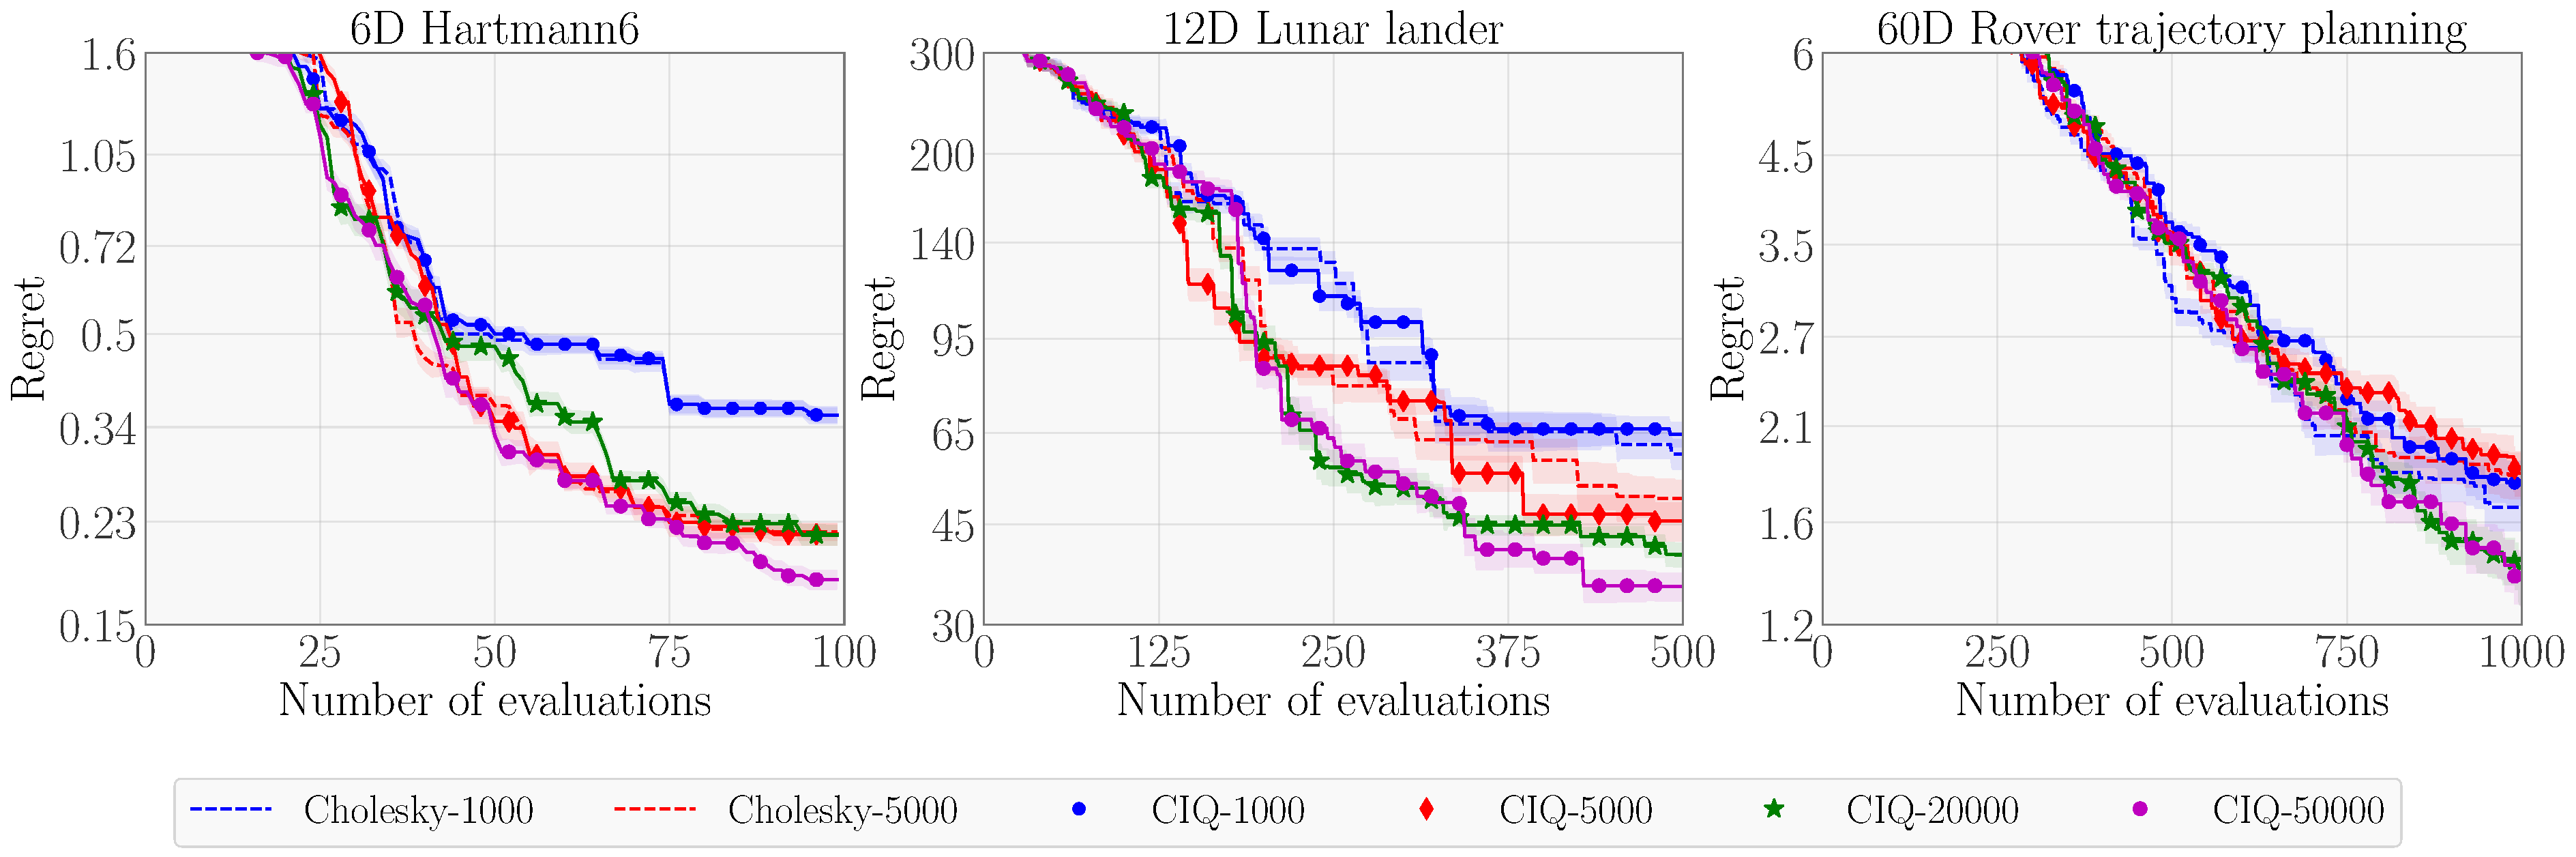
\includegraphics[width=\linewidth]{figures/bo_ciq.pdf}
  \caption[
    Comparison of msMINRES-CIQ versus other sampling methods for Bayesian optimization via Thompson Sampling.
  ]{
    A comparison of sampling methods for Bayesian Optimization (BO).
    BO is applied to the ({\bf left}) Hartmann ($D=6$) and ({\bf right}) Lunar Lander ($D=12$) problems.
    Methods: Cholesky-$\langle T \rangle$ draws posterior samples with Cholesky at $T$ candidate points.
    CIQ-$\langle T \rangle$ draws posterior samples with msMINRES-CIQ.
    RFF-50k uses random Fourier features to draw approximate posterior samples at $50,\!000$ candidate points.
    Larger $T$ results in better optimization.
    msMINRES-CIQ enables scaling to $T \geq 50,\!000$.
    Each plot shows mean regret with standard error in log-scale based on 30 replications.
  }
  \label{fig:bayesopt}
\end{figure}

\paragraph{Experimental details.}
The 6-dimensional {\bf Hartmann} function is a classical test problem in global optimization\footnote{\url{https://www.sfu.ca/~ssurjano/hart6.html}}.
There are 6 local minima and a global minimum with value $-3.32237$.
We use a total of 100 evaluations with 10 initial points.
The 10 initial points are generated using a Latin hypercube design and we use a batch size of 5.
In each iteration, we draw 5 samples and select 5 new trials to evaluate in parallel.

We consider the same setup and controller as in \cite{eriksson2019scalable} for the 12-dimensional {\bf Lunar Lander} problem\footnote{
 From the Open-AI gym: \url{https://gym.openai.com/envs/LunarLander-v2}
}.
The goal is to learn a controller that minimizes fuel consumption and distance to a given landing target while also preventing crashes.
The state of the lunar lander is given by its angle and position, and their time derivatives.
Given this state vector, the controller chooses one of the following four actions: $a \in \{\text{do nothing, booster left, booster right, booster down}\}$.
The objective is the average final reward over a fixed constant set of $50$ randomly generated terrains, initial positions, and initial velocities.
The optimal controller achieves an average reward of $\approx 309$ over the 50 environments.

For both problems, we use a Mat\'ern-$5/2$ kernel with ARD and a constant mean function.
The domain is scaled to \smash{$[0, 1]^d$} and we standardize the function values before fitting the Gaussian process.
The kernel hyperparameters are optimized using L-BFGS-B and we use the following bounds: (lengthscale) $\ell \in [0.01, 2.0\,]$, (signal variance) $s^2 \in [0.05, 50.0]$, (noise variance) $\sigma^2 \in [1e-6, 1e-2]$.
Additionally, we place a horseshoe prior on the noise variance as recommended in \cite{snoek2012practical}.
We add $1\mathrm{e}{-4}$ to the diagonal of the kernel matrix to improve the conditioning and use a preconditioner of rank $200$ for CIQ.


\paragraph{Baselines.}
We measure the performance of TS as a function of the candidate set size $T$ and consider $T \in \{ 1,\!000, 5,\!000, 20,\!000, 50,\!000 \}$.
We run Cholesky ({\bf Cholesky}-$T$) for  $T \in \{ 1,\!000, 5,\!000\}$ and msMINRES-CIQ ({\bf CIQ}-$T$) for $T \ge 5,\!000$.
Note that it would be very challenging and impractical to use Cholesky with $T \geq 10,\!000$, due to its quadratic memory and cubic time complexity.
In addition to Cholesky and CIQ with exact Gaussian processes as the surrogate model, we also compare to random Fourier features (RFF) \cite{rahimi2008random} with $1,\!000$ random features.

\paragraph{Optimization performance.}
We plot the mean regret with standard error based on 30 replications in \cref{fig:bayesopt}.
By increasing $T=1,\!000$ to $T=50,\!000$, the final regret achieved by CIQ is significantly lower on both problems.
%We re-iterate that $T=50,\!000$ is largely impractical with Cholesky.
Large candidate sets have previously only been possible with approximate sampling methods like RFF.
We note, however, that RFF with $T=50,\!000$ is outperformed by CIQ-50k on both problems.
